% This is a simple LaTex sample document that gives a submission format
%   for IEEE PAMI-TC conference submissions.  Use at your own risk.

% Make two column format for LaTex 2e.
\documentclass[10pt,twocolumn]{article}
\usepackage{times}
\usepackage{picinpar}
\usepackage{epsfig}
\usepackage{graphicx}
\usepackage{amsmath}
\usepackage{amsfonts}
%\usepackage{photo}
\usepackage{fancyhdr}
\usepackage{lastpage}
\pagestyle{fancy}
\fancyhead{}
\lhead{Team \#17343}
\rhead{Page \thepage \,of \pageref{LastPage}}
\cfoot{}

\fancyfootoffset{0pt}

% Use following instead for LaTex 2.09 (may need some other mods as well).
% \documentstyle[times,twocolumn]{article}

% Set dimensions of columns, gap between columns, and paragraph indent 
\setlength{\textheight}{8.875in}
\setlength{\textwidth}{6.875in}
\setlength{\columnsep}{0.3125in}
\setlength{\topmargin}{0in}
\setlength{\headheight}{12.0pt}
\setlength{\headsep}{0in}
\setlength{\parindent}{1pc}
\setlength{\oddsidemargin}{-.1875in}  % Centers text.
\setlength{\evensidemargin}{-.1875in}

% Add the period after section numbers.  Adjust spacing.
\newcommand{\Section}[1]{\vspace{-8pt}\section{\hskip -1em.~~#1}\vspace{-3pt}} 
\newcommand{\SubSection}[1]{\vspace{-3pt}\subsection{\hskip -1em.~~#1}
     	\vspace{-3pt}}

\renewcommand{\headrulewidth}{0pt}
\renewcommand{\voffset}{10pt}

\begin{document}

% Don't want date printed
\date{}

% Make title bold and 14 pt font (Latex default is non-bold, 16pt) 
\title{\bf MCM 2012.B}

% For single author (just remove % characters)
\author{Team \#17343}

% For two authors (default example)
%\author{\begin{tabular}[t]{c@{\extracolsep{8em}}c} 
%I. M. Anonymous  & M. Y. Coauthor \\
% \\
%        My Department & Coauthor Department \\
%        My Institute & Coauthor Institute \\
%        City, STATE~~zipcode & City, STATE~~zipcode
%\end{tabular}}

\maketitle
\thispagestyle{fancy}

\section*{\centering Abstract}

{\em
Given a river with $Y$ campsites distributed uniformly along its length, herein is investigated the problem of scheduling six to eighteen day long river rafting trips down the river over the 180 day rafting season so as to maximize campsite usage and minimize contact between rafting groups. The problem is approached by allocating maximal usage of campsites by initially scheduling the maximum possible number of eighteen day trips, using all campsites maximally, and using decomposing transformations to swap, for example, an eighteen day trip with two consecutive nine day trips, without sacrificing neither the initial property of maximal usage nor lack of contact between groups. A matrix encoding these decomposition transformations and each of their effects is used in combination with simulated annealing to find the optimal solution with respect to the given constraints.
}

\tableofcontents

\Section{Introduction}
We are tasked with the problem of maximizing the number of river rafting trips of length six to eighteen days down the 225 mile long Big Long River where each night of the trip is spent in one of $Y$ campsites distributed uniformly along the river; constraints are that each campsite is to host at most one group of rafters per night and that contact between groups is to be minimized. The schedule of trips offered throughout a 180-day season are all to be scheduled preemptively and rafters are to be given either oar powered boats, which travel at four miles per hour on average, or motor powered boats, which travel at eight miles per hour on average.

An optimal solution is to have all $Y$ campsites occupied every day of the season (aside from the ones that cannot be reached immediately on the opening day or following several days) with no river rafting group ever seeing another on the river.

\Section{Definitions}
\SubSection{Campsite Numbering and Division}
Refer to the $i$th campsite as $c_i$, $i = 1, \dotsc, Y$. A trip along the river can last at most 18 days, so, given that there are $Y$ campsites, define $n = \left\lfloor \frac{Y}{18} \right\rfloor$ and $r = Y \mod 18 \nonumber$ so that $Y = 18n + r$. with $0 < n$ and $0 \leq r < n$. Let $T_k$ refer to a trip down the river that takes $k$ days.

\SubSection{Trip Transformations}
Consider a trip $T_{18}$ down the river that visits campsites some sequence of eighteen campsites. $T_{18}$ can be subdivided into two trips of shorter length that visit the same set campsites over the same eighteen days:

\begin{align}
x_1: T_{18} &\rightarrow \{T_{6}, T_{12}\} \nonumber\\
x_2: T_{18} &\rightarrow \{T_{7}, T_{11}\} \nonumber\\
x_3: T_{18} &\rightarrow \{T_{8}, T_{10}\} \nonumber\\
v_4: T_{18} &\rightarrow \{T_{9}, T_{9}\} \nonumber
\end{align}

Transformations $x_1,\dotsc, x_4$ only generate trips six to twelve day trips. Two simultaneous trips $T_{18}$ that depart on the same day and visit disjoint subsets of the set of campsites can be broken down into three shorter trips such that one of the three generated shorter trips has length $13$ to $17$.

To form a trip $T_{k}$ with $k \in [13,17] \cap \mathbb{Z}$, if $k = k_1 + k_2$ where $k_1,k_2 \in [6,12] \cap \mathbb{Z}$, two trips $T_{18}$ can be transformed into three trips $T_k$, $T_{18-k_1}$, and $T_{18-k_2}$: 

\begin{align}
x_5: 2 * T_{18} &\rightarrow \{T_{11}, T_{12}, T_{13}\} \nonumber\\
x_6: 2 * T_{18} &\rightarrow \{T_{10}, T_{12}, T_{14}\} \nonumber\\
x_7: 2 * T_{18} &\rightarrow \{T_{11}, T_{11}, T_{14}\} \nonumber\\
x_8: 2 * T_{18} &\rightarrow \{T_{9}, T_{12}, T_{15}\} \nonumber\\
x_9: 2 * T_{18} &\rightarrow \{T_{10}, T_{11}, T_{15}\} \nonumber\\
x_{10}: 2 * T_{18} &\rightarrow \{T_{8}, T_{12}, T_{16}\} \nonumber\\
x_{11}: 2 * T_{18} &\rightarrow \{T_{9}, T_{11}, T_{16}\} \nonumber\\
x_{12}: 2 * T_{18} &\rightarrow \{T_{10}, T_{10}, T_{16}\} \nonumber\\
x_{13}: 2 * T_{18} &\rightarrow \{T_{7}, T_{12}, T_{17}\} \nonumber\\
x_{14}: 2 * T_{18} &\rightarrow \{T_{8}, T_{11}, T_{17}\} \nonumber\\
x_{15}: 2 * T_{18} &\rightarrow \{T_{9}, T_{10}, T_{17}\} \nonumber
\end{align}

Finally, a trip $T_{18}$ can be broken down into three shorter trips in only one way,

$$x_{16}: T_{18} \rightarrow \{T_6, T_6, T_6\}$$

for if $18 = k_1 + k_2 + k_3$ with each $k_i$ initially at $6$, increasing any of the $k_i$ has to be accompanied with decreasing another $k_j$ below $6$, and no trips of length less than six days are allowed.

\SubSection{Transformation Matrix}
Define a $12 \times 16$ matrix $T$ such that entry $T_{i,j}$ corresponds to how many trips of length $5+i$ are created by transformation $x_j$:
\begin{align}
&T = \nonumber\\
&\left[\begin{array}{cccccccccccccccc}
1 & 0 & 0 & 0 & 0 & 0 & 0 & 0 & 0 & 0 & 0 & 0 & 0 & 0 & 0 & 3 \\
0 & 1 & 0 & 0 & 0 & 0 & 0 & 0 & 0 & 0 & 0 & 0 & 1 & 0 & 0 & 0 \\
0 & 0 & 1 & 0 & 0 & 0 & 0 & 0 & 0 & 1 & 0 & 0 & 0 & 1 & 0 & 0 \\
0 & 0 & 0 & 2 & 0 & 0 & 0 & 1 & 0 & 0 & 1 & 0 & 0 & 0 & 1 & 0 \\
0 & 0 & 1 & 0 & 0 & 1 & 0 & 0 & 1 & 0 & 0 & 2 & 0 & 0 & 1 & 0 \\
0 & 1 & 0 & 0 & 1 & 0 & 2 & 0 & 1 & 0 & 1 & 0 & 0 & 1 & 0 & 0 \\
1 & 0 & 0 & 0 & 1 & 1 & 0 & 1 & 0 & 1 & 0 & 0 & 1 & 0 & 0 & 0 \\
0 & 0 & 0 & 0 & 1 & 0 & 0 & 0 & 0 & 0 & 0 & 0 & 0 & 0 & 0 & 0 \\
0 & 0 & 0 & 0 & 0 & 1 & 1 & 0 & 0 & 0 & 0 & 0 & 0 & 0 & 0 & 0 \\
0 & 0 & 0 & 0 & 0 & 0 & 0 & 1 & 1 & 0 & 0 & 0 & 0 & 0 & 0 & 0 \\
0 & 0 & 0 & 0 & 0 & 0 & 0 & 0 & 0 & 1 & 1 & 1 & 0 & 0 & 0 & 0 \\
0 & 0 & 0 & 0 & 0 & 0 & 0 & 0 & 0 & 0 & 0 & 0 & 1 & 1 & 1 & 0
\end{array}\right] \nonumber
\end{align}

Given a $16$-row column vector $c$, whose element $c_i$ denotes how many times to employ transformation $x_i$, $Tc$ calculates how many trips of lengths six through seventeen days will be created. Let

\begin{align}
&R = (-1, -1, -1, -1, \nonumber\\
&-2, -2, -2, -2, -2, -2, -2, -2, -2, -2, -2, -1)\nonumber
\end{align}

so that element $i$ of $R$ denotes how many trips of length 18 are decomposed by transformation $x_i$. If there are initially $k$ trips of length 18, applying the transformations encoded in column vector $c$ leaves in $k - Rc$ trips of length 18. More succinctly, let $d$ be a $13$-row column vector so that $d_i = (Tc)_i$ for $i = 1, \dotsc, 12$ and $d_13 = k - Rc$; $d_i$ encodes the number of trips of length $5 + i$ scheduled after the application of the transformations denoted in $c$.

%This is not a square matrix. A brute-force search found that avoiding transformations $x_2$, $x_3$, $x_6$ and $x_8$ and leaves a nonsingular matrix; call this matrix $T$.

%$$T = \left[\begin{array}{cccccccccccc}
%1 & 0 & 0 & 0 & 0 & 0 & 0 & 0 & 0 & 0 & 0 & 3 \\
%0 & 0 & 0 & 0 & 0 & 0 & 0 & 0 & 1 & 0 & 0 & 0 \\
%0 & 0 & 0 & 0 & 0 & 1 & 0 & 0 & 0 & 1 & 0 & 0 \\
%0 & 2 & 0 & 0 & 0 & 0 & 1 & 0 & 0 & 0 & 1 & 0 \\
%0 & 0 & 0 & 0 & 1 & 0 & 0 & 2 & 0 & 0 & 1 & 0 \\
%0 & 0 & 1 & 2 & 1 & 0 & 1 & 0 & 0 & 1 & 0 & 0 \\
%1 & 0 & 1 & 0 & 0 & 1 & 0 & 0 & 1 & 0 & 0 & 0 \\
%0 & 0 & 1 & 0 & 0 & 0 & 0 & 0 & 0 & 0 & 0 & 0 \\
%0 & 0 & 0 & 1 & 0 & 0 & 0 & 0 & 0 & 0 & 0 & 0 \\
%0 & 0 & 0 & 0 & 1 & 0 & 0 & 0 & 0 & 0 & 0 & 0 \\
%0 & 0 & 0 & 0 & 0 & 1 & 1 & 1 & 0 & 0 & 0 & 0 \\
%0 & 0 & 0 & 0 & 0 & 0 & 0 & 0 & 1 & 1 & 1 & 0
%\end{array}\right]$$
%$$\det(T) = -18 \neq 0$$

\Section{Solution}
Allocate $n$ trips of length 18 departing each of the first 162 days of the rafting season (an 18 day trip departing later will not reach the end of the river before season end) so that the $k$th trip on a given day stops at campsites $c_{k + nm}$ on day $m$; there are $162n$ trips allocated. Consider the equation $Tc = t$ with $T$ from the previous section and $t$ a 12-row column vector whose $i$th element designates the number of trips of length $5+i$ that are desired. Use simulated annealing to solve for the closest solution for $c$ with $c$'s elements constrained to be integers by minimizing $||Tc - t||$. Applying transformation $x_i$ $c_i$ will produce trips of various trip lengths closest to the desired distribution and leave $162n - Rc$ trips of length 18.

Since trips shorter than 18 days are created by decomposing trips from a schedule that occupies all campsites every night of the season, the generated schedule is maximally uses available resources for the first 162 days. The remaining 18 days will be considered later as they do not allow allocation of 18 day trips.

\SubSection{A Simplifying Assumption}
The given problem will be solved for the case $Y = 18n$, that is, it will be momentarily assumed that the number of campsites along the river is a multiple of 18; this assumption will later be lifed and solved for. 

\SubSection{Proof of Optimality}
\paragraph{$x_1, \dotsc, x_4$}
Consider a series of 18 campsites $c_1, \dotsc, c_{18}$, each occupied by a rafter group $r_i$. Let movement to position $c_{19}$ designate exiting the river. Group $r_i$ is to proceed to campsite $c_j$ the next day, where $i < j \leq 19$ with no two $r_i$ going to the same $c_j$.

If a new group of rafters $s$ taking an 18-day trip is to depart on the next day, $c_1$ will be available, $c_2$ the next day, and so on, group $s$ will be able to complete its trip. Suppose that $s$'s 18 day trip is composed into two shorter trips, $p$ and $q$, so that $q$ departs when $p$ has completed its trip. If $p$ goes to campsite $c_1$ on the first day, nothing needs to be done. On the other hand, suppose that $p$ is to camp at $c_k$ for some $k > 1$ on the first day. The group at $c_l$ for some $l < k$ is scheduled to proceed to camp at $c_k$ on the same day. Have the group at $c_l$ remain there for an additional night and allocate $c_k$ to group $p$. On the day after, the camp that the group at $c_l$ would have reached in two days is empty, so have the group at $c_l$ proceed to that now empty camp instead. Schedule around $p$'s second day in a way analogous to what was just done. As $q$ will proceed down the river only once $p$ has exited the river, the same scheduling algorithm can be used for $q$. All campsites are used every day and are occupied by at most one rafter group at once.

If rescheduling a neighboring camp site's current group's itinerary in order to allow a shorter trip to overtake them will produce a collision between the stalled group and another group, simply apply the rescheduling algorithm recursively to eliminate the problems.

\begin{center}
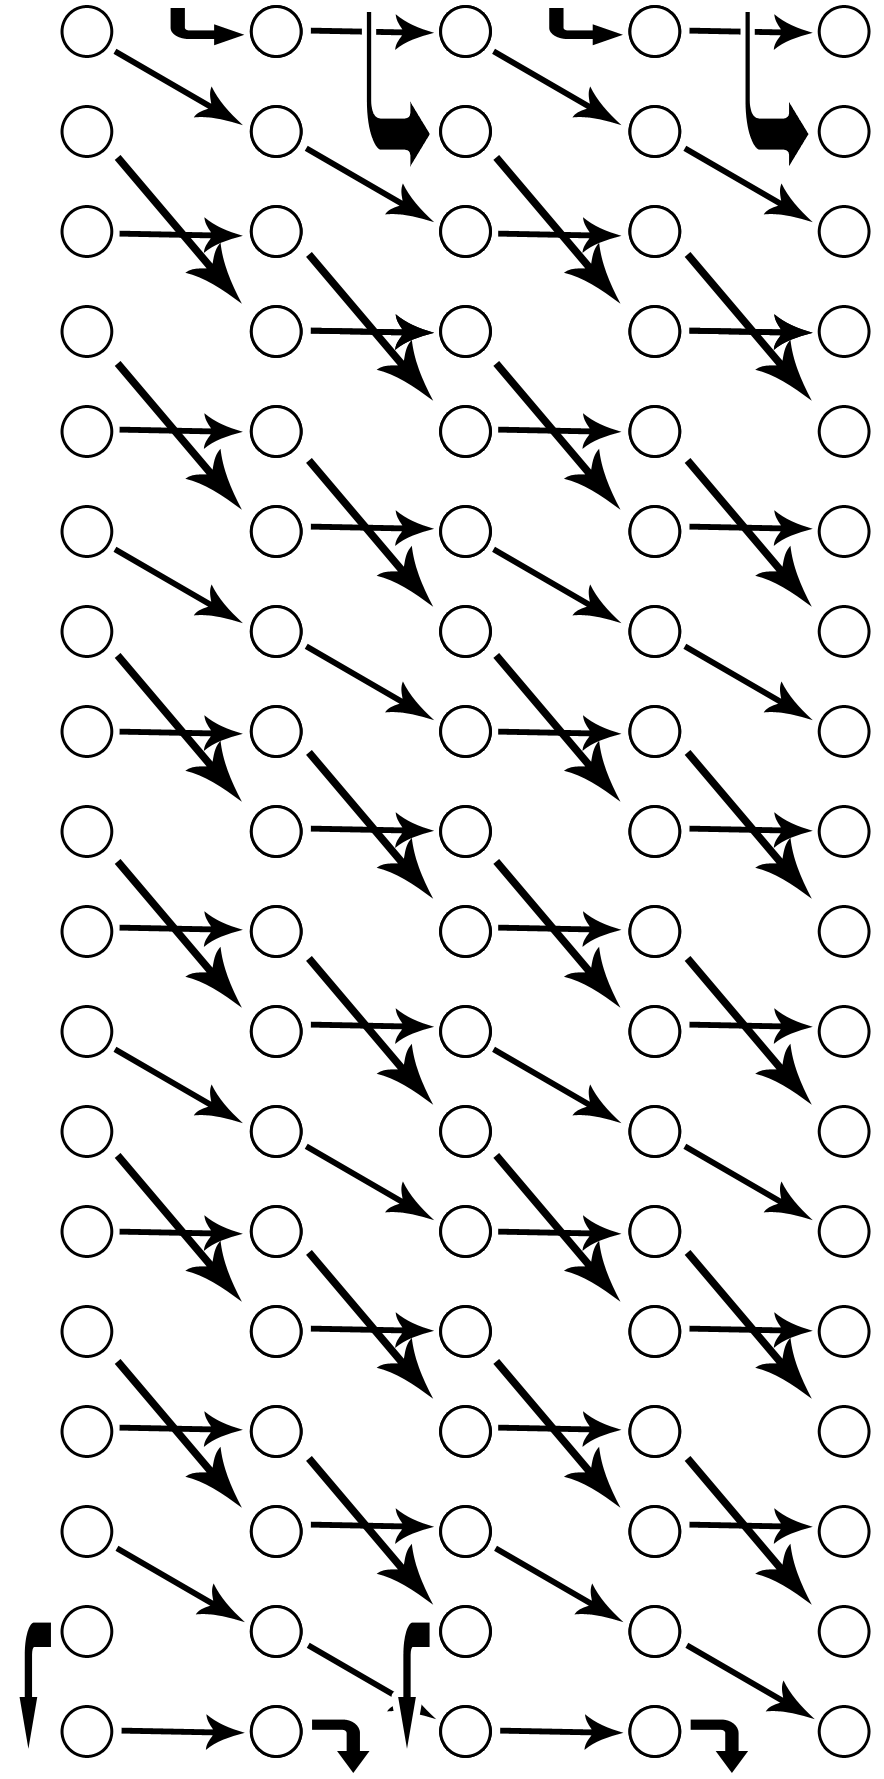
\includegraphics[width=2.5in]{img/1.png}\newline
\emph{Fig. 1: An example of a rescheduled itinerary for a group of 18 camps over four days.}
\end{center}

\paragraph{$x_5, \dotsc, x_{16}$}
In the case of two 18 day trips being decomposed to three trips, note that the tree trips are constructed by decomposing one 18-day trip into two shorter trips $r_1$ and $r_2$, the other into two shorter trips $s_1$ and $s_2$, and then (without loss of generality) combining $r_1$ with $s_2$ into a longer trip $t$ and leaving $r_2$ and $s_1$ as shorter trips. Reorder $t$ so that the campsites are in order of increasing distance down the river and leave $r_2$ and $s_1$ unchanged to preserve optimality without inducing campsite occupancy collisions.

\SubSection{Boat Assignment}
Since stalling a group by one night and having it proceed in one day to where it would normally have arrived in two days will double the amount of distance necessary for that group to travel, assign stalled groups powerboats instead of oarboats (since powerboats move twice as quickly as oarboats) in order to guarantee that their itineraries are possible.

\SubSection{Minimizing Camper Contact}
Note in the above rescheduling algorithm that whenever one campgroup overtakes another on the river as a result of being scheduled on a shorter trip, the campgroups being overtaken remain at their campsites while being passed. Thus, a camping group should never run into another group while rafting. Camper contact is therefore kept to the minimum of zero.

\SubSection{Removing the Simplifying Assumption}
Recall that it was assumed that the number of campsites $Y$ is a multiple of 18. In reality, there will be $r$ campsites left over, where $0 \leq r \leq 17$. This can be solved by adding the $i$th leftover campsite as an additional night to the trips of the groups that will be in the $i$th of the last $Y - (Y \mod 18)$ trips. When using the simulated annealing method, adjust accordingly by decreasing by one the entries in the target vector corresponding to the numbers of trips of length $18 - r$ or greater. If any of these numbers are already zero, leave them zero; optimality will be preserved at the expense of accuracy with respect to desired distribution of numbers of trips of each length.

\SubSection{The Last 18 Days}
Recall that the original assignment of trips was to give $n$ trips of length 18 days on each of the first 162 days of the season. These last 18 days can be put to use by assigning $n$ trips of length $18 - i$ on day $162 + i$ for $i = 1, \dotsc, 12$; it is not possible to offer a trip beginning later than the 174th day because it would extend past the end of the rafting season.

Once these $12n$ trips have been assigned, a model analogous to the one given so far can be constructed by finding decomposition transformations of trips of lengths 12 through 17, $T_k$ for $k = 12, \dotsc, 17$. Rename $T$, $c$, $t$, $R$,and $d$ to $T_{18}$, $c_{18}$, $t_{18}$, $R_{18}$, and $d_{18}$, respectively; construct twelve additional copies for the cases of 12 through 17 day trips and, analogously, name them using the same letters but with subscripts $11 + i$ for $i = 1, \dotsc, 6$; alter the new variables as appropriate (e.g. $(d_12)_12 = n - R_kc_k$); and alter the simulated annealing implementation to minimize

$$\left|\left|c - \left(\sum_{k=6}^{18} T_kt_k\right)\right|\right|$$

where $c$ is the vector whose $i$th element encodes the desired number of trips of length $5+i$, $i = 1\dotsc,13$. This completed model will ensure maximum possible usage of all campsites for all 180 days of the rafting season.

\Section{An Example (Preliminary) Result}
Suppose that an equal number of trips of lengths 6 through 17. The basic model which does not account for the last 18 days or for a number of campsites not equal to a multiple of 18 was implemented in Mathematica (see Appendix for code) - these details, though solved theoretically above, could not be accounted for due to time constraints - and was used to solve this case:

\begin{align}
c &= \{0, 1, 4, 3, 2, 1, 4, 4, 2, 4, 1, 3, 7, 2, 1, 4\} \nonumber\\
d &= \{12, 8, 10, 12, 14, 16, 18, 2, 5, 6, 8, 10, 88\} \nonumber
\end{align}

This gives a total of 209 trips throughout the season. Note that the disparity between the desired number of trips and the solution found is partly due to lack of implementation for the entire model and partly due to the goal of maximal daily usage of campsites; a better result would likely be achieved.

\Section{Analysis and Discussion}
The model presented allows one to decide what distribution of trip lengths is desired and find the closest possible solution that maintains maximum possible camp utilization while keeping contact between groups to zero. As the model begins with an optimal schedule and alters it via transformations that preserve optimality, there is no way to have greater campsite utilization; since contact on the river is already zero, it cannot be further reduced. Boat assignment is also optimal as it ensures that rescheduled itineraries are possible to fulfill.

The only drawback of the proposed model is that it generally does not allow one to achieve the exact numbers of trips of each possible trip length that are desired as doing so would generally leave some campsites empty and destroy the maximality of the solution. The discrepancy can be nontrivial, as illustrated by the example given in the previous section.

\Section{Possible Model Extension}
The task considered here is that of optimally making use of the campsites along the river. If the main priority is changed to succeeding in scheduling exactly the number of trips of each length that is desired, the given model will not suffice. However, it can be used to find the closest solution to the desired distribution of trips, after which additional trip decomposition transformations could be used that generate only one shorter trip of a desired length could be used to sacrifice optimality in favor of accuracy.

\newpage

\Section{Appendix: Mathematica Code}
\begin{verbatim}
ZZ = {
{1, 0, 0, 0, 0, 0, 0, 0, 0, 0, 0, 0, 0, 0, 0, 3},
{0, 1, 0, 0, 0, 0, 0, 0, 0, 0, 0, 0, 1, 0, 0, 0},
{0, 0, 1, 0, 0, 0, 0, 0, 0, 1, 0, 0, 0, 1, 0, 0},
{0, 0, 0, 2, 0, 0, 0, 1, 0, 0, 1, 0, 0, 0, 1, 0},
{0, 0, 1, 0, 0, 1, 0, 0, 1, 0, 0, 2, 0, 0, 1, 0},
{0, 1, 0, 0, 1, 0, 2, 0, 1, 0, 1, 0, 0, 1, 0, 0},
{1, 0, 0, 0, 1, 1, 0, 1, 0, 1, 0, 0, 1, 0, 0, 0},
{0, 0, 0, 0, 1, 0, 0, 0, 0, 0, 0, 0, 0, 0, 0, 0},
{0, 0, 0, 0, 0, 1, 1, 0, 0, 0, 0, 0, 0, 0, 0, 0},
{0, 0, 0, 0, 0, 0, 0, 1, 1, 0, 0, 0, 0, 0, 0, 0},
{0, 0, 0, 0, 0, 0, 0, 0, 0, 1, 1, 1, 0, 0, 0, 0},
{0, 0, 0, 0, 0, 0, 0, 0, 0, 0, 0, 0, 1, 1, 1, 0}};

"Desired number of trips of length 6,7,...,18"
CC = {15, 15, 15, 15, 15, 15, 15, 15, 15, 15, 15, 15};

"simulated annealing finds the solution that gets closet to CC"
x = {aa, bb, cc, dd, ee, ff, gg, hh, ii, jj, kk, ll, mm, nn, oo, pp};
y = x /. Last[
   NMinimize[{(ZZ.x - CC).(ZZ.x - 
        CC), (aa | bb | cc | dd | ee | ff | gg | hh | ii | jj | kk | 
         ll | mm | nn | oo | pp) \[Element] Integers && aa >= 0 && 
      bb >= 0 && cc >= 0 && dd >= 0 && ee >= 0 && ff >= 0 && gg >= 0 && 
      hh >= 0 && ii >= 0 && jj >= 0 && kk >= 0 && ll >= 0 && mm >= 0 && 
      ll >= 0 && oo >= 0 && pp >= 0}, x, 
    Method -> "SimulatedAnnealing", MaxIterations -> 10000]]

"Gives the number of trips of length 6,7,...,17 after transformations \
have been applied"
ZZ.y

"remaining number of trips of length 18"
z = 162 + {-1, -1, -1, -1, -2, -2, -2, -2, -2, -2, -2, -2, -2, -2, \
-2, -1}.y

"Double check that our trips still add up to 162 trips of 18 days each"
sum = z*18 + {6, 7, 8, 9, 10, 11, 12, 13, 14, 15, 16, 17}.(ZZ.y)
\end{verbatim}


%\begin{thebibliography}{9}
%\small  % Use 9 point text.
%\bibitem{model:url}
%Team \#11604. ``Anastasds/mcm2010 - GitHub.'' MCM 2010 Problem B Model Implementation. 13 Feb. 2011. Web. 13 Feb. 2011. $\langle$ https://github.com/anastasds/mcm2010 $\rangle$.

%\bibitem{discussion:att}
%"How Does a Cell Tower Squeeze so Much into a T1? - Cellphones, Providers, and Plans | DSLReports Forums.'' DSLReports Home : Broadband ISP Reviews News Tools and Forums. 22 Sept. 2000. Web. 13 Feb. 2011. $\langle$ http://www.dslreports.com/forum/r5595012-How-does-a-Cell-Tower-squeeze-so-much-into-a-T1-$\rangle$.

%\bibitem{csbook}
%Sedgewick, Robert. \textit{Algorithms in C$++$. Reading, Mass.: Addison-Wesley Publishing Company, 1992. Print.}

%\end{thebibliography}

%{\footnotesize
%}

%\begin{biography}{Anastas Stoyanovsky}
%\end{biography}


\end{document}
